\renewcommand\chaptername{}
\chapter{DATA AND METHODOLOGY}

\section{Study area}

Geographical location of the experimental area is shown in Figure \ref{StudyArea}. The forests, which are located in Ust-Ilimsky district, Itkutsk oblast (southeastern Siberia, 31N and 64E approximately), are classified as boreal deciduous, the terrain is pretty plain, with minor gently sloping areas. 
This choice of the study area was due to the fact that there was already an ongoing work on logging and forest inventory. Besides, trees in this area are good representatives of the majority of all forest stands in the region and characterize their diversity quite well, so the results of the model will have good generalization for the region. 

10 RGB-camera mounted drone flights were performed on the experimental region. Total area covered by the \gls{UAV}s is 1020 hectares (Figure \ref{StudyArea}), 486 hectares out of the total amount was used in dataset generation.\\

\begin{figure}[ht]
\centering
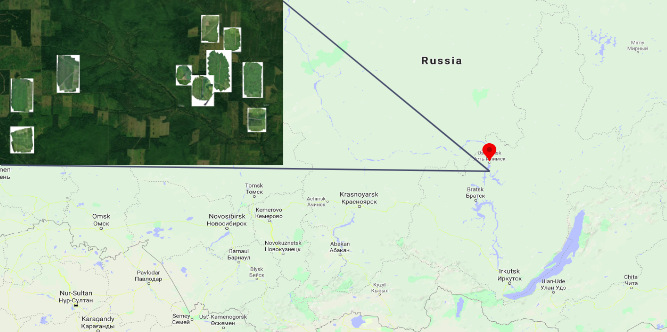
\includegraphics[scale=0.7]{images/StudyArea.png}
\caption{Geographical location of the experimental area}
\label{StudyArea}
\end{figure}

\section{Dataset generation}

The orthophotos and \gls{DSM} files of the 10 experimental regions were processed and stitched using the Agisoft Metashape software from the raw RGB images, obtained from the drone. Agisoft Metashape is a special software product, which performs photogrammetric processing of digital images and generates spatial data. Aerial RGB orthophoto resolution was around 0.05m, \gls{DSM} images resolution varies from 0.1m to 0.2m. After that, 10 rectangular polygons were cut from the original orthophotos and \gls{DSM} files, due to the reason that the quality of photogrammetry at the edges of the images were lower, and contained artifacts. This happens due to the fact that the amount of overlapping images at the edges is significantly lower in comparison to the middle part, and the software cannot obtain proper orthographic view. However, the off-nadir imagery with different perspective views are also highly useful for diversity of the data, since most of the satellite imagery is collected from the off-nadir perspective, thus we tried to make the rectangular polygons as big as possible. 

Next step was to obtain the ground truth masks of delineated trees from the \gls{DSM} files. From the \gls{DSM} raster image (first image of Figure \ref{DataGen}a) we can clearly observe the round shapes, which correspond to the tree crowns on RGB orthophotos. The main idea was to create 3 segmentation masks, which correspond to Individual trees, Background and Boundary (between the trees, or between the trees and background). Individual trees mask is binary raster image, where distinct contours are the tree crowns, background is the mask with non-forested region in the images. Firstly, non-forested area needs to be thresholded from the \gls{DSM}. This would be trivial if we had \gls{CHM} rasters, or the terrain had no curvature and slope, however in our case we need to perform terrain flattening operation. This can be done by applying Flat-field correction technique, which can be performed by subtracting the Gaussian blurred image from the original one. Thereby we create pseudo flat field reference image, by correcting the illumination intensity levels. After that, the background is thresholded from the forested regions. By applying the Local maxima method highest points of tree crowns are determined from the thresholded forestry regions (Figure \ref{DataGen}b), then using these points as markers we apply the Watershed algorithm to delineate the tree crowns from each other (Figure \ref{DataGen}c). This is how we obtain the needed masks from \gls{DSM} raster images. Different mathematical morphological operations, such as adaptive histogram equalization, erosion, dilation, opening and closing, etc., were used in the process. The main challenge here is that all of the operations were performed by visual observation and interpretation of the obtained masks, since, as it was addressed in Section 2.2, the proper delineation can be made only by accurate selection of parameters for all of the mentioned algorithms. Most of the proposed algorithms and methods were carried out using the Skimage and OpenCV libraries.

\begin{figure}[ht]
\centering
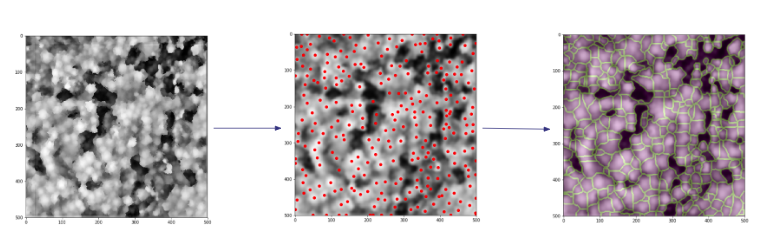
\includegraphics[scale=0.6]{images/DataGen.png}
\caption{The process of dataset generation. a) \gls{DSM}  raster image, b) Local maxima of \gls{DSM}, c) Watershed tree delineation} 
\label{DataGen}
\end{figure}

The final step of dataset generation pipeline was to rescale the RGB aerial orthophotos and ground truth masks to match the satellite imagery spatial resolutions (0.5m and 0.31m). The number of trees for every experimental area is presented in Table \ref{TreeN}, it can be seen that the number of trees slightly differs for different resolutions. Important issue to note here is the thickness of the boundaries: too thick boundaries lead to decrease or loss of the tree crown area. On the other hand, some part of thin boundaries will disappear in the rescaled ground truth masks.  Moreover, too thin boundaries may not be enough for deep neural network to perform the proper tree delineation. The optimal boundary thickness for 0.5m resolution was 2-3 pixels, for 0.31m resolution 3-4 pixels. Overall, 10 polygons of aerial imagery were processed by proposed methodology, and rescaled to corresponding spatial resolutions.


\begin{table}
\caption{Number of trees (contours) in ground truth masks delineated from the aerial imagery}
\label{TreeN}
\vskip 0.15in
\begin{center}
\begin{small}
\begin{sc}
\begin{tabular}{|l|p{4cm}|p{4cm}|}
\hline
\textbf{Experimental area} & \textbf{Number of trees in 0.31m rescaled ground truth} & \textbf{Number of trees in 0.5m rescaled ground truth}\\\hline
Region1 &18481  & 18478\\\hline
Region2 &20876  & 20485\\\hline
Region3 &5167  & 5171\\\hline
Region4 &15534  & 15487\\\hline
Region5 &14259  & 14220\\\hline
Region6 &19090  & 19089\\\hline
Region7 &14829  & 14820\\\hline
% Region8 &  & \\\hline
Region9 &5871  & 5875\\\hline
Region10 &7335  & 7327\\\hline
\end{tabular}
\end{sc}
\end{small}
\end{center}
\vskip -0.1in
\end{table}

\section{Deep neural network: model training}

Deep convolutional neural network is state-of-the-art method for object detection and segmentation in RGB imagery. For our particular case U-Nets with ResNet Encoders and cross connections was chosen, since this is currently one of the most popular architectures for semantic and instance segmentation tasks, showing decent results in different competitions. Convolutional networks can be substantially deeper, more accurate, and more efficient to train if they contain shorter connections between layers close to the input and those close to the output. Thus, the backbone of this architecture is build on Residual Networks \gls{ResNet} with 34 layers, which is made from a series of residual blocks with skip connections (Figure \ref{CNN} (left)), so basically ResNet is used for the encoder/down sampling part of our architecture. Model with 34 layers was chosen to be optimal for our dataset in terms of training time and memory consumption. 

\begin{figure}[ht]
\centering
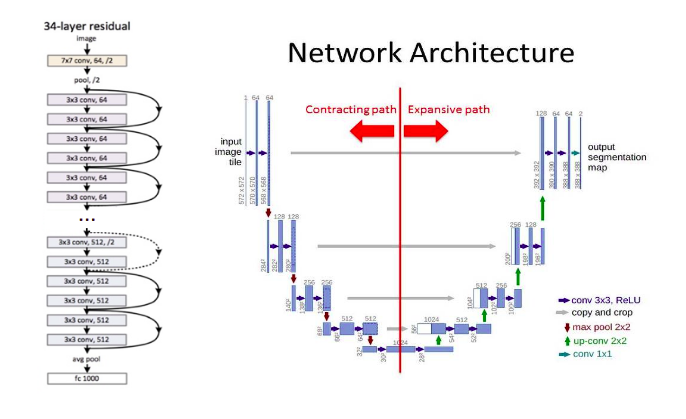
\includegraphics[scale=0.7]{images/CNNArch.png}
\caption{\gls{ResNet} (left) and \gls{Unet} (right) architectures
} 
\label{CNN}
\end{figure}


The decoding part of our \gls{CNN} is U-Net architecture, which initially was developed for biomedical image segmentation. U-Nets have been found to be very effective for tasks where the output is of similar size as the input and the output needs that amount of spatial resolution. This makes them very good for creating segmentation masks and for image processing/generation.
The \gls{Unet} is used for the upsampling, where the reverse of the downsampling path is carried out to retain the original image resolution.

The initial model was created from Segmentation Models library (Python library with Neural Networks for Image Segmentation based on Keras and TensorFlow). Initially, the model was pre-trained for 2-class segmentation task to classify forest/non-forest regions with 2m spatial resolution imagery. Then the model structure was changed to perform 3-class segmentation task (tree, boundary, background) for \gls{ITC} delineation, retaining the weights of pre-trained model. This procedure is know as transfer learning, where the knowledge (weights) for some task is obtained, and then applied to related problem. By doing so we can significantly improve the model efficiency and training time. 

The initial dataset imagery, containing 10 experimental regions of interest \gls{ROI} was divided into 30 images of smaller size, shuffled, and then split into Train/Validation/Test datasets with 70/20/10 percentages. Since entire images cannot fit into GPU memory, 256*256 pixel size batches were used to provide enough spatial context for tree delineation, solving the memory constraints. The model with batch size of 16  was trained on nVidia GeForce GTX 1080Ti for 100 epochs. Different types of image augmentations were used from Albumentations library. The loss function used for training is Categorical Cross-Entropy, which is basically combination of Softmax activation function and Cross-Entropy loss. The metrics used for training the model are Intersection over Union \gls{IoU} and F1 score.
These are the most common used metrics for semantic segmentation. \gls{IoU}, also known as the Jaccard Index, is calculated by the following formula:

\begin{eqnarray*}
\text{\gls{IoU}} & = & \frac{\text{Area of Overlap}}{\text{Area of Union}}
\end{eqnarray*}

For multi-class segmentation, the mean IoU of the image is calculated by taking the IoU of each class and averaging them. 

F1 score, also known as the Dice Coefficient, is calculated by the following formula:

\begin{eqnarray*}
\text{F1 score} & = & \frac{\text{Area of Overlap}}{\text{Total number of pixels combined}}
\end{eqnarray*}


Model evaluation is done by standard segmentation metrics, described above, plus 2 custom metrics, which are 1) Number of trees (contours) comparison between the ground truth and predicted images, 2) Tree detection rate, where the tree centers points from ground truth are obtained and checked if they fall inside the predicted tree contours.



